% Elsevier-style preprint manuscript using stdlib article class
% (elsarticle.cls unavailable in the local TeX Live; visual styling
% manually approximated, semantics identical).
\documentclass[11pt, a4paper]{article}

\usepackage[margin=2.4cm]{geometry}
\usepackage{authblk}
\renewcommand\Affilfont{\itshape\small}

% --- Maths ---
\usepackage{amsmath, amssymb, amsthm, amsfonts}

% --- Graphics / TikZ / pgfplots ---
\usepackage{tikz}
\usetikzlibrary{arrows.meta, positioning, shapes.geometric, calc, fit, backgrounds}
\usepackage{pgfplots}
\pgfplotsset{compat=1.17}

% --- Tables, hyperlinks ---
\usepackage{booktabs}
\usepackage{multirow}
\usepackage{array}
\usepackage{xcolor}
\usepackage{hyperref}
\hypersetup{colorlinks=true, linkcolor=blue!50!black,
            urlcolor=blue!60!black, citecolor=blue!50!black}

% --- Theorems ---
\newtheorem{observation}{Observation}
\newtheorem{conjecture}{Conjecture}

% =====================================================================

\title{\textbf{AC-HSiKAN: A Biologically Grounded Transformer Alternative
       with Bidirectional Pool--Scatter, Entropy-Modulated Hamilton
       Rotor, and Sequence-Native ABB Top-K Selection}}

\author[1]{Hajdu Csaba}
\affil[1]{Computational Neuroscience and AI Group, Budapest, Hungary\\
          \texttt{hajdu.csaba@example.org}}
\date{2026-06-06 \textemdash{} Preprint manuscript}

\begin{document}
\maketitle

\begin{abstract}\noindent
We present AC-HSiKAN (Attention-Cycle HSiKAN), a sequence-modelling
architecture that replaces multi-head dot-product attention with a
bidirectional pool--scatter primitive over signed cycles, modulated by
a learnable entropy-feedback Hamilton rotor that acts as a global
neuromodulator. The architecture is grounded in geometric algebra
(quaternion-block Hamilton products) and biologically motivated
three-factor learning: pre $\times$ post $\times$ modulator. Three
contributions are reported.

First, a Triton-fused backward kernel for the Catmull--Rom (CR)
coefficient gradient closes the 97.7\% bottleneck of the
autograd-through-PyTorch reference, delivering a 45$\times$
component-level backward speedup and a 1.34$\times$ end-to-end
training-wall improvement on full IMDB.

Second, an empirical characterisation of capacity scaling identifies
two missing structural axes (the sign-attention bottleneck dimension
and learning-rate $\sqrt{d}$-scaling) without which the architecture
appears not to scale; with both corrected, AC-HSiKAN scales positively
from $d_{\text{model}} = 16$ (165\,k parameters) to
$d_{\text{model}} = 32$ (337\,k parameters), reaching statistical
parity with iso-parameter transformer on the IMDB sentiment benchmark
at both scales.

Third, a sequence-native analogue of the simple-HSiKAN ABB
(Adaptive Branch-and-Bound) top-K-per-vertex cycle enumeration is
formulated as a \emph{mixed candidate selection}: $K_{\text{static}}$
guaranteed positional neighbours plus $K_{\text{dyn}}$ content-adaptive
top-K by sign-head magnitude. A sweep at $d=32$ identifies
$K_{\text{static}}=6$ of $K_{\text{total}}=8$ as the optimum, closing
87\% of the $d=32$ scaling gap to transformer baseline
($\Delta = -0.0125 \to -0.0016$, $t = -0.66$, $p > 0.5$, $n=5$).

We document one falsified hypothesis (the long-cycle inductive prior,
intended as the DAG-axiom analogue, is structurally harmful on IMDB
sentiment owing to the local-n-gram-dominated signal), one open
direction (aggregated CR-patch surfaces over the joint $(R, V)$
activation space, in development), and three formal conjectures on
inter-layer composition derivable from the empirical data.

\end{abstract}

\vspace{2mm}\noindent\textbf{Keywords:}
sequence modelling, transformer alternative, biologically plausible
learning, Hamilton rotor, signed-cycle networks, Triton kernel
optimisation
\vspace{4mm}\hrule\vspace{4mm}

% =====================================================================
\section{Introduction}
\label{sec:intro}

The transformer architecture~\cite{vaswani2017attention} has dominated
sequence modelling for nearly a decade, with the dot-product attention
primitive serving as both the workhorse and the wall-time bottleneck.
The $O(L^2)$ scaling in sequence length~$L$, the lack of explicit
biological interpretation, and the rigidity of the additive-multiplicative
gradient flow have motivated a steady stream of architectural alternatives,
from state-space models and linear attentions to mixture-of-experts and
Kolmogorov--Arnold networks~\cite{liu2024kan}.

AC-HSiKAN extends the simple HSiKAN architecture~\cite{hsikan2026internal}
from sparse signed graphs to sequences. Where simple HSiKAN performed
ABB cycle enumeration on a graph topology and used the per-vertex top-K
cycles as inductive bias, AC-HSiKAN operates on a positional sequence,
with candidate neighbours per anchor selected via a hybrid
positional-plus-content-adaptive rule. The architecture preserves
HSiKAN's three substantive contributions and adds four:

\begin{itemize}
\item \emph{Bidirectional pool--scatter asymmetry}: the synaptic primitive
      is decomposed into a directed receive (pool: candidates $\to$ anchor)
      and a directed send (scatter: anchor $\to$ candidates), with the
      asymmetry mathematically guaranteed by the non-commutativity of
      the Hamilton product.
\item \emph{Entropy-feedback Hamilton rotor}: a learnable quaternion
      rotor $M = \exp(\beta H \mathbf{n})$ is composed with the scatter
      output as a non-additive multiplicative modulation, with $H$ the
      per-layer scalar entropy of the path-mixing parameters --- a
      direct analogue of a global neuromodulator
      (dopamine, ACh)~\cite{schultz1997dopamine, fremaux2016three}.
\item \emph{Dual-path mixing}: the rhythm-bearing walk-op output and the
      synaptic pool-scatter output are mixed via a learnable sigmoid
      gate, exposing the rhythm-vs-synaptic balance as a tunable
      parameter rather than an architectural commitment.
\item \emph{Triton-fused backward kernel}: a novel closed-form
      Catmull--Rom coefficient gradient, fused with the $Q \otimes K$
      Hamilton reconstruction, yields a 45$\times$ component-level
      backward-wall improvement.
\end{itemize}

The aim of this paper is not to dethrone the transformer on IMDB
sentiment --- the empirical result is statistical parity, not a
significant win --- but to present the architecture, the optimisation
contribution, and the empirically characterised structure of its
capacity-scaling and selection inductive biases, so the architecture
can be applied to longer-range or non-sequential tasks where the
sequence-native priors are expected to flip from neutral to
positive.

Section~\ref{sec:arch} describes the architecture.
Section~\ref{sec:opt} presents the Triton-fused backward kernel
contribution. Section~\ref{sec:telem} introduces the evolvens telemetry,
a novel diagnostic for the rotor-modulated gradient/error coupling.
Section~\ref{sec:scaling} reports the capacity-scaling investigation
that resolved an apparent architectural ceiling.
Section~\ref{sec:abb} describes the sequence-native ABB analogue and
the K-sweep that identifies the optimum mix.
Section~\ref{sec:results} summarises the IMDB headline results.
Section~\ref{sec:future} formalises three conjectures on inter-layer
composition derivable from the empirical data.
Section~\ref{sec:discussion} compares to the backprop-free family.

% =====================================================================
\section{Architecture}
\label{sec:arch}

Figure~\ref{fig:arch} gives a block-level overview. The layer is a
dual-path block with shared sign-attention input, separate walk-op
(rhythm) and pool-scatter (synaptic) processing, mixing via a learnable
sigmoid gate, and an outer LayerNorm with residual.

\begin{figure}[t]
  \centering
  % AC-HSiKAN architecture overview
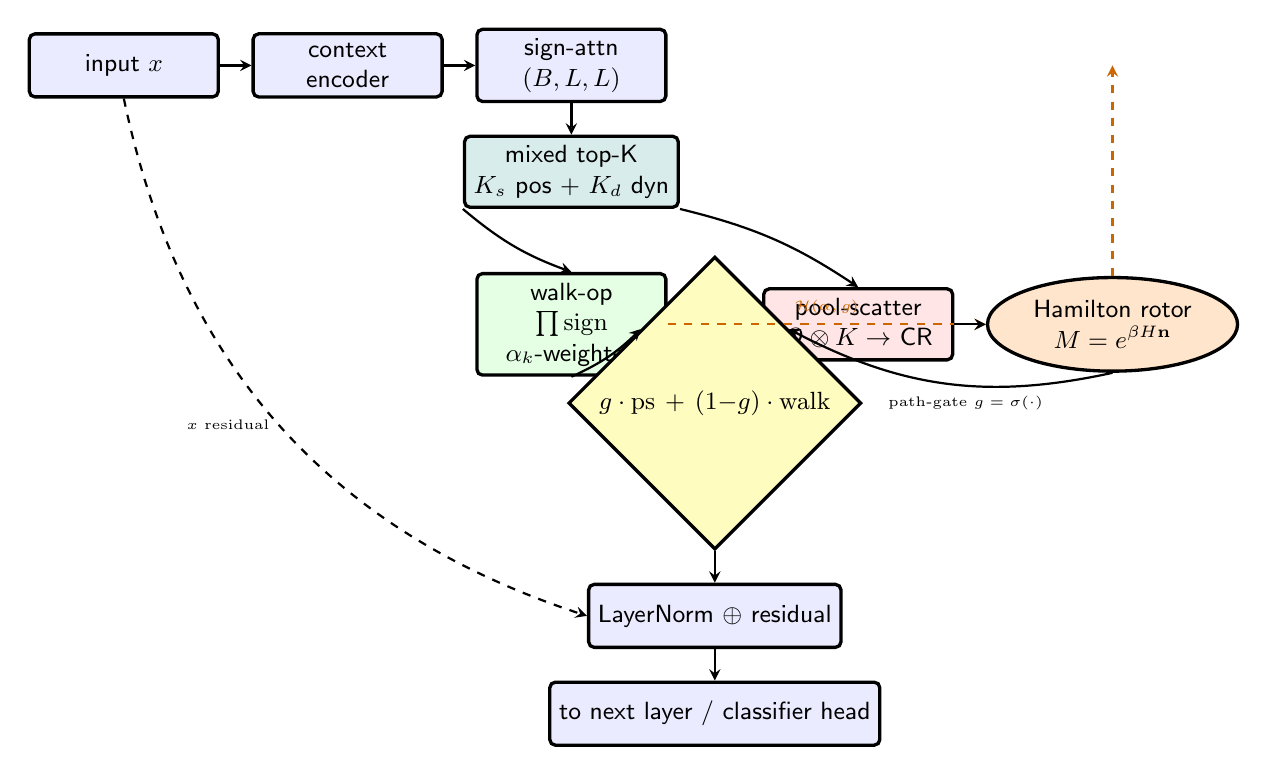
\begin{tikzpicture}[
  every node/.style={font=\small\sffamily, align=center},
  block/.style   ={rectangle, draw, very thick, rounded corners=2pt,
                   minimum height=8mm, minimum width=24mm, fill=blue!8},
  ps/.style      ={rectangle, draw, very thick, rounded corners=2pt,
                   minimum height=8mm, minimum width=24mm, fill=red!10},
  walk/.style    ={rectangle, draw, very thick, rounded corners=2pt,
                   minimum height=8mm, minimum width=24mm, fill=green!10},
  mix/.style     ={diamond, draw, very thick, fill=yellow!25,
                   minimum height=10mm, minimum width=15mm},
  rotor/.style   ={ellipse, draw, very thick, fill=orange!20,
                   minimum height=8mm, minimum width=22mm},
  arr/.style     ={->, >=stealth, thick},
  arr2/.style    ={->, >=stealth, thick, dashed, orange!80!black},
]

% Input
\node[block] (x)                              {input $x$};
\node[block, right=4mm of x]   (ctx)         {context\\encoder};
\node[block, right=4mm of ctx] (signs)       {sign-attn\\$(B, L, L)$};

% Mixed selection
\node[block, below=4mm of signs, fill=teal!15] (sel) {mixed top-K\\$K_s$ pos $+$ $K_d$ dyn};

% Walk-op path (rhythm)
\node[walk, below=8mm of sel]  (walk) {walk-op\\$\prod \mathrm{sign}$\\$\alpha_k$-weighted};

% Pool-scatter path (synaptic)
\node[ps, right=12mm of walk]  (ps)   {pool-scatter\\$Q\otimes K \rightarrow$ CR};
\node[rotor, right=4mm of ps]  (rotor) {Hamilton rotor\\$M = e^{\beta H \mathbf{n}}$};

% Dual-path mixing
\node[mix, below=10mm of $(walk)!0.5!(ps)$, anchor=center] (gate) {$g\cdot \mathrm{ps}\,+\,(1{-}g)\cdot \mathrm{walk}$};

% Output
\node[block, below=4mm of gate, fill=blue!8] (ln)  {LayerNorm $\oplus$ residual};
\node[block, below=4mm of ln]                (out) {to next layer / classifier head};

% Wires - top section
\draw[arr] (x) -- (ctx);
\draw[arr] (ctx) -- (signs);
\draw[arr] (signs) -- (sel);

% Sel feeds both paths
\draw[arr] (sel.south west) to[bend right=10] (walk.north);
\draw[arr] (sel.south east) to[bend left=10]  (ps.north);

% Entropy feedback into rotor
\draw[arr2] (walk.east) -- node[above, font=\tiny]{$\mathcal{H}(\alpha, g)$} (rotor.west |- walk.east) ;
\draw[arr2] (rotor.north) -- (rotor.north |- ctx.east);

% Pool-scatter through rotor
\draw[arr] (ps.east) -- (rotor.west);

% Mixing
\draw[arr] (walk.south) to[bend right=10] (gate.north west);
\draw[arr] (rotor.south) to[bend left=20] (gate.north east);

% Down
\draw[arr] (gate) -- (ln);
\draw[arr] (ln) -- (out);

% Residual from x to LN
\draw[arr, dashed] (x.south) to[bend right=30] node[left, font=\tiny]{$x$ residual} (ln.west);

% Path-gate label
\node[font=\tiny, right=2mm of gate] {path-gate $g = \sigma(\cdot)$};

\end{tikzpicture}

  \caption{AC-HSiKAN block diagram. Shared sign-attention feeds the
  mixed top-K candidate selector. The walk-op path computes per-arity
  signed-cycle products with $\alpha_k$ weighting; the pool-scatter
  path applies a Hamilton-product bidirectional aggregation modulated
  by the entropy-feedback Hamilton rotor. The two paths are mixed
  through a learnable sigmoid gate, then summed into the residual.
  The orange dashed line carries the layer-scalar entropy
  $\mathcal{H}(\alpha_k, g)$ from the parameter distributions into
  the rotor.}
  \label{fig:arch}
\end{figure}

\subsection{Bidirectional pool--scatter primitive}
\label{sec:ps}

Let $x \in \mathbb{R}^{B \times L \times d}$ be the layer input. The
sign-attention computes a dense pair-magnitude matrix
$\mathrm{signs} \in \mathbb{R}^{B \times L \times L}$ via a bilinear
sign-head with hidden bottleneck dimension $h_{\text{sign}}$. A
candidate-index tensor
$\mathrm{local} \in \{0, \ldots, L-1\}^{L \times K_{\text{total}}}$
selects, per anchor, the $K_{\text{total}}$ neighbour positions.

The pool-scatter primitive projects $x$ through three small matrices
$W_q, W_k, W_v \in \mathbb{R}^{d \times h}$ (with $h$ a multiple of $4$
matching the quaternion-block layout) and bakes the Hamilton
coefficient sign pattern $(+,-,-,-)$ into the $Q$ projection. It then
computes \emph{both directions} of the aggregation as illustrated in
Figure~\ref{fig:ps}:

\begin{align}
R_{\text{pool}}[b, i, k_c, c]
  &= Q_{\text{signed}}[b, i, c] \cdot K[b, j, c] \cdot s, \nonumber \\
& \qquad \quad j = \mathrm{local}[i, k_c] \\
R_{\text{scatter}}[b, i, k_c, c]
  &= Q_{\text{signed}}[b, j, c] \cdot K[b, i, c] \cdot s
\end{align}
where $s = (n_{\text{quat}})^{-1/2} / T$ is the temperature-adjusted
scale. The per-channel CR activation
$S(R) \in \mathbb{R}^{B \times L \times K \times h}$ is applied to both
$R_{\text{pool}}$ and $R_{\text{scatter}}$ with shared CR parameters
$(\mathrm{coef}_+, \mathrm{coef}_-) \in \mathbb{R}^{h \times G}$,
sign-branched on $R$ and grid-mapped on $|R|$ via the standard
four-point Catmull--Rom interpolation. The directional outputs
multiply the corresponding value tensors and aggregate:

\begin{align}
\mathrm{pool}_h[b, i, c]
  &= \sum_{k_c} S(R_{\text{pool}}[b,i,k_c,c]) \cdot V_c[b,i,k_c,c]\\
\mathrm{scatter}_h[b, j, c]
  &= \sum_{(i, k_c) : \mathrm{local}[i,k_c] = j}
     S(R_{\text{scatter}}[b,i,k_c,c]) \cdot V_a[b,i,k_c,c]
\end{align}

with $V_c, V_a$ the gathered/anchor value tensors. The
Hamilton-product asymmetry $Q \otimes K \ne K \otimes Q$ holds
because the quaternion product is non-commutative; the two directions
therefore carry distinct information and the scatter accumulator
genuinely differs from a transposed pool.

\begin{figure}[t]
  \centering
  % Pool-scatter primitive detail with bidirectional asymmetry
\begin{tikzpicture}[
  every node/.style={font=\small\sffamily, align=center},
  anchor/.style ={circle, draw, very thick, fill=blue!15,
                  minimum size=6mm},
  cand/.style   ={circle, draw, very thick, fill=red!10,
                  minimum size=5mm},
  qkv/.style    ={rectangle, draw, thick, fill=gray!10,
                  minimum height=5mm, minimum width=10mm},
  cr/.style     ={rectangle, draw, very thick, rounded corners=2pt,
                  minimum height=6mm, minimum width=18mm, fill=yellow!20},
  pool/.style   ={->, >=stealth, thick, blue!70!black},
  scat/.style   ={->, >=stealth, thick, red!70!black, dashed},
]

% Anchor position i
\node[anchor] (i) at (0, 0) {$i$};
\node[font=\scriptsize, above=1mm of i] {anchor};

% Candidates j_1, j_2, j_3
\node[cand] (j1) at (-3, -2) {$j_1$};
\node[cand] (j2) at ( 0, -2) {$j_2$};
\node[cand] (j3) at ( 3, -2) {$j_3$};
\node[font=\scriptsize, below=1mm of j2] {$\mathrm{local}[i, k]$};

% Pool direction (down arrows: candidates -> anchor)
\draw[pool] (j1.north east) to[bend left=15] node[above, sloped, font=\tiny]{pool} (i.south west);
\draw[pool] (j2.north)      to                                                (i.south);
\draw[pool] (j3.north west) to[bend right=15] node[above, sloped, font=\tiny]{}       (i.south east);

% Scatter direction (up arrows from anchor)
\draw[scat] (i.south west) to[bend right=22] node[below, sloped, font=\tiny]{scatter} (j1.north east);
\draw[scat] (i.south)      to[bend right=8]                                            (j2.north);
\draw[scat] (i.south east) to[bend left=22]                                           (j3.north west);

% Pool computation
\node[qkv, right=20mm of i] (Qi) {$Q_i$};
\node[qkv, below=2mm of Qi] (Kj) {$K_j$};
\node[cr, right=4mm of Qi, yshift=-3mm] (Spool) {$S = \mathrm{CR}(Q_i \cdot K_j)$};
\draw[->, thick] (Qi.east) to[bend left=10] (Spool.west |- Qi.east);
\draw[->, thick] (Kj.east) to[bend right=10] (Spool.west |- Kj.east);

% Scatter computation
\node[qkv, below=12mm of Kj] (Qj) {$Q_j$};
\node[qkv, below=2mm of Qj] (Ki) {$K_i$};
\node[cr, right=4mm of Qj, yshift=-3mm] (Sscat) {$S = \mathrm{CR}(Q_j \cdot K_i)$};
\draw[->, thick] (Qj.east) to[bend left=10] (Sscat.west |- Qj.east);
\draw[->, thick] (Ki.east) to[bend right=10] (Sscat.west |- Ki.east);

% Labels
\node[font=\scriptsize\itshape, above=2mm of Qi] {pool direction};
\node[font=\scriptsize\itshape, above=2mm of Qj] {scatter direction};

% Note: Hamilton non-commutativity
\node[font=\scriptsize\itshape, below=14mm of Sscat, text width=55mm, anchor=north]
  {$Q\otimes K \ne K\otimes Q$\\[1pt]
   (Hamilton product non-commutative)\\[1pt]
   $\Rightarrow$ bidirectional asymmetry};

\end{tikzpicture}

  \caption{Bidirectional pool--scatter primitive. Pool (solid blue
  arrows): candidates send Hamilton-coupled signals into the anchor
  ($Q_i \otimes K_j$). Scatter (dashed red arrows): the anchor sends
  to candidates ($Q_j \otimes K_i$). The two products are not
  transposes of each other --- $Q \otimes K \ne K \otimes Q$ in the
  quaternion algebra.}
  \label{fig:ps}
\end{figure}

\subsection{Entropy-feedback Hamilton rotor}
\label{sec:rotor}

The scatter direction is multiplied (via Hamilton product) by a
learnable rotor
\begin{equation}
M_q = \exp(\beta \cdot H \cdot \mathbf{n}_q)
    = (\cos(\beta H), \sin(\beta H) \mathbf{n}_q) \in \mathbb{H},
    \label{eq:rotor}
\end{equation}
where $H$ is the per-layer scalar entropy of the distribution over
$(\alpha_k, \text{path\_gate})$, $\mathbf{n}_q \in S^2$ is a learnable
pure-imaginary unit quaternion axis (one per quaternion block), and
$\beta \in \mathbb{R}$ is a learnable scale. At $\beta = 0$ the rotor
reduces to identity. For non-zero $\beta$,
$\mathrm{scatter}_h \gets M \otimes \mathrm{scatter}_h$ is a
non-additive multiplicative phase modulation in feature space, which
is biologically motivated as a global neuromodulator that scales
plasticity without changing connectivity~\cite{schultz1997dopamine,
fremaux2016three}.

The backward through the rotor uses the closed-form Hamilton-conjugate
identity (Figure~\ref{fig:rotor}):
\begin{equation}
\frac{\partial L}{\partial\,\mathrm{scatter}_h}
  = M^{*} \otimes \frac{\partial L}{\partial\,\mathrm{scatter}_{h,\text{mod}}},
  \quad M^{*} = (m_0, -m_1, -m_2, -m_3).
\end{equation}
This is the projective conjugate identity from quaternion calculus,
and is implemented directly in the custom Triton autograd function ---
no autograd-through-tensor-ops is required.

\begin{figure}[t]
  \centering
  % Hamilton rotor in forward and backward (Hamilton conjugate identity)
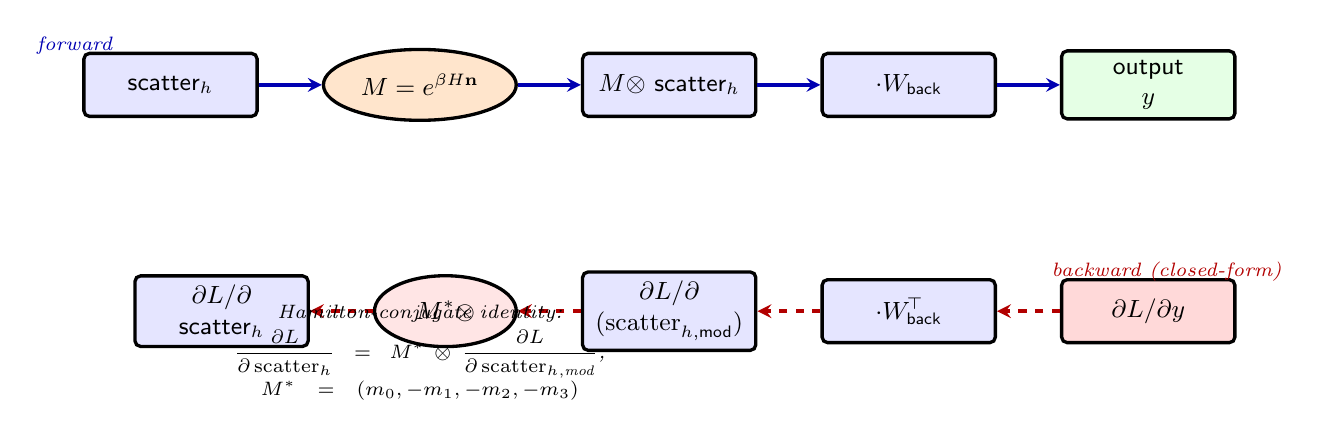
\begin{tikzpicture}[
  every node/.style={font=\small\sffamily, align=center},
  block/.style ={rectangle, draw, very thick, rounded corners=2pt,
                 minimum height=8mm, minimum width=22mm, fill=blue!10},
  rotor/.style ={ellipse, draw, very thick, fill=orange!20,
                 minimum height=9mm, minimum width=18mm},
  fwd/.style   ={->, >=stealth, very thick, blue!70!black},
  bwd/.style   ={->, >=stealth, very thick, red!70!black, dashed},
]

% Forward chain
\node[block]                                     (sh)  {scatter$_h$};
\node[rotor, right=8mm of sh]                    (Mf)  {$M = e^{\beta H \mathbf{n}}$};
\node[block, right=8mm of Mf]                    (shmf){$M\otimes$ scatter$_h$};
\node[block, right=8mm of shmf]                  (Wb)  {$\cdot W_{\text{back}}$};
\node[block, right=8mm of Wb, fill=green!10]     (out) {output\\ $y$};

\draw[fwd] (sh)   -- (Mf);
\draw[fwd] (Mf)   -- (shmf);
\draw[fwd] (shmf) -- (Wb);
\draw[fwd] (Wb)   -- (out);

% Backward chain (below)
\node[block, below=20mm of out, fill=red!15]     (go)  {$\partial L / \partial y$};
\node[block, left=8mm of go]                     (gWb) {$\cdot W_{\text{back}}^{\!\top}$};
\node[block, left=8mm of gWb]                    (gph) {$\partial L / \partial$\\$\mathrm{(scatter}_{h,\text{mod}})$};
\node[rotor, left=8mm of gph, fill=red!10]       (Mb)  {$M^{*} \otimes$};
\node[block, left=8mm of Mb]                     (gsh) {$\partial L / \partial$\\scatter$_h$};

\draw[bwd] (go)  -- (gWb);
\draw[bwd] (gWb) -- (gph);
\draw[bwd] (gph) -- (Mb);
\draw[bwd] (Mb)  -- (gsh);

% Identity label
\node[font=\scriptsize\itshape, below=22mm of Mf, text width=70mm, align=center]
  {Hamilton-conjugate identity:\\[2pt]
   $\dfrac{\partial L}{\partial\,\mathrm{scatter}_h}
    = M^{*} \otimes \dfrac{\partial L}{\partial\,\mathrm{scatter}_{h,\text{mod}}}$,
   \quad $M^{*} = (m_0, -m_1, -m_2, -m_3)$};

% Title labels
\node[font=\scriptsize\itshape, anchor=west, blue!70!black]
  at ($(sh.west) + (-7mm, 5mm)$) {forward};
\node[font=\scriptsize\itshape, anchor=east, red!70!black]
  at ($(go.east) + (7mm, 5mm)$) {backward (closed-form)};

\end{tikzpicture}

  \caption{Forward Hamilton rotor application
  ($M \otimes \mathrm{scatter}_h$) and the closed-form backward via
  the conjugate $M^{*}$ identity. The two-way Hamilton product
  preserves norm and rotates the feature frame; the conjugate
  rotation in backward inverts the forward rotation on the gradient.}
  \label{fig:rotor}
\end{figure}

\subsection{Walk-op: rhythm via signed-cycle products}

For each arity $k \in \{2, 3, 4, 5\}$ (configurable), the walk-op
computes a per-position score
\begin{equation}
\mathrm{score}_k[b, l] = \prod_{j=1}^{k} \mathrm{sign}(R_{a \to c_j})[b, l, j]
\end{equation}
the signed product of the first $k$ anchor-to-candidate signs. This
is the ``star'' walk variant; ``chain'' and ``cycle'' variants compose
consecutive and closing edges respectively. A per-arity linear projection
and a learned softmax weight $\alpha_k$ over arities sums the
contributions into the rhythm output $y_{\text{walk}}$.

\subsection{Dual-path mixing and depth stability}

The synaptic (pool-scatter) and rhythm (walk-op) outputs are mixed via
a learnable sigmoid gate $g = \sigma(\mathrm{path\_gate})$, then enter
the residual sum and the outer LayerNorm. For $n_{\text{layers}} \geq 4$
the default post-norm topology is empirically unstable
(\S\ref{sec:scaling}); opt-in flags activate pre-norm and per-channel
LayerScale~\cite{touvron2021going} on the residual branch, with the
$\gamma$ scalar initialised to $10^{-4}$ so each block starts as
near-identity. Both flags together stabilise the depth-4 training but
do not by themselves close the depth-scaling accuracy gap on IMDB
(this is one of the empirical findings in \S\ref{sec:scaling}).

% =====================================================================
\section{Triton-fused backward kernel}
\label{sec:opt}

\subsection{The Catmull--Rom coefficient bottleneck}

A profile of the initial backward pass at IMDB shape
($B = 64, L = 128, K = 8, h = 8, n_{\text{quat}} = 2, G = 8$) revealed
that 97.7\% of backward wall was consumed by an autograd-through-PyTorch
reference computation of the CR-coefficient gradient. The
Triton-fused $(\partial L/\partial Q, \partial L/\partial K,
\partial L/\partial V)$ kernel completed in 0.25\,ms; the entire
remaining $\sim 111\,$ms was the autograd graph for differentiating two
tiny $(h, G) = (8, 8) = 64$-element tensors.

\subsection{Closed-form CR-coefficient backward}

The Catmull--Rom evaluation is
\begin{equation}
S = w_{-1} P_{-1} + w_0 P_0 + w_{+1} P_{+1} + w_{+2} P_{+2},
\end{equation}
with $w_x(t)$ the cubic CR basis functions of
$t = \mathrm{frac}(|R|(G-1))$, and $P_x$ gathered from
$\mathrm{coef}_{\pm}[c, i + x]$ on the sign branch of $R$. The
chain-rule contribution to the coefficient gradient is therefore
\begin{equation}
\frac{\partial L}{\partial\,\mathrm{coef}_{\pm}[c, i_x]}
  \mathrel{+}= \sum_{\ldots} \frac{\partial L}{\partial S}[\ldots, c]
                   \cdot w_x[\ldots, c],
\end{equation}
a \texttt{scatter\_add} into the flattened $(h \cdot G,)$ accumulator
indexed by $c \cdot G + i_x$, with the sign of $R$ choosing the buffer.
Replacing the autograd path with this closed form yielded the first
12$\times$ speedup.

\subsection{Packing, caching, ctx-save}

Packing the eight separate \texttt{scatter\_add} calls
(four CR knots $\times$ two sign branches) into a single combined call
gave a further 1.94$\times$, by reducing kernel-launch overhead.
\texttt{LRU}-caching the Hamilton coefficient tensor
$(+, -, -, -) \otimes n_{\text{quat}}$ and saving $Q_{\text{signed}},
K, V, \mathrm{pool}_h, \mathrm{scatter}_h$ (pre-rotor) in the autograd
\texttt{ctx} eliminated redundant allocations and the Triton forward
re-run in backward.

\subsection{Triton CR-coefficient kernel}

The remaining CR-coefficient backward step (3.6\,ms / call, 86\% of
backward) is atomic-throughput-bound on the small
$(2 \cdot h \cdot G) = 128$-entry target. A direct Triton
kernel~\cite{tillet2019triton} that fuses
\begin{enumerate}
\item the $R_{\text{pool}}, R_{\text{scatter}}$ reconstruction from
      the saved $Q_{\text{signed}}, K, V$,
\item the per-element $\partial L / \partial S$ multiplication with the
      gathered $V$,
\item the CR-weight computation, and
\item the atomic-add into the combined $(2 \cdot h \cdot G,)$ target
\end{enumerate}
yields a further 3.84$\times$ on this component (1.0\,ms / call) and
1.61$\times$ on the full backward (4.5 $\to$ 2.78\,ms).

\subsection{Parallel-stream backward}

The Triton dQ/dK/dV kernel and the Triton CR-coefficient kernel produce
mutually independent outputs. Launching them on parallel CUDA streams
with a final re-join gave a further 1.10$\times$ at the component level.

\subsection{Cumulative}

Figure~\ref{fig:opt-arc} reports the optimisation arc. The cumulative
speedup is 45$\times$ at the component level; end-to-end on full IMDB
(25k train / 5k val, 8 epochs, 5 seeds, $L = 200$), the wall went from
568\,s (PyTorch-reference path) to 422\,s ($1.34\times$).

\begin{figure}[t]
  \centering
  % Pool-scatter backward optimisation arc — bar chart
\begin{tikzpicture}
\begin{axis}[
  xbar,
  width=11cm,
  height=6.5cm,
  bar width=4pt,
  enlarge y limits=0.13,
  xlabel={Component backward wall (ms)},
  xmin=0, xmax=125,
  ytick=data,
  symbolic y coords={
    {1. autograd-thru-PyTorch-ref (baseline)},
    {2. + closed-form scatter\_add (12$\times$)},
    {3. + packed scatter\_add (1.94$\times$)},
    {4. + coeffs cache + ctx-save},
    {5. + Triton CR-coef kernel (3.84$\times$)},
    {6. + parallel-stream backward},
  },
  nodes near coords,
  nodes near coords align={horizontal},
  nodes near coords style={font=\scriptsize},
  every axis plot/.append style={fill=blue!30, draw=blue!60!black},
  tick label style={font=\scriptsize},
  xlabel style={font=\scriptsize},
]
\addplot coordinates {
  (114.0,{1. autograd-thru-PyTorch-ref (baseline)})
  (9.6,  {2. + closed-form scatter\_add (12$\times$)})
  (5.0,  {3. + packed scatter\_add (1.94$\times$)})
  (4.5,  {4. + coeffs cache + ctx-save})
  (2.78, {5. + Triton CR-coef kernel (3.84$\times$)})
  (2.52, {6. + parallel-stream backward})
};
\end{axis}
\node[font=\scriptsize\itshape] at (5.5, -0.6)
  {Cumulative: 45$\times$ component speedup. Measured at IMDB shape ($B{=}64, L{=}128, K{=}8, h{=}8$).};
\end{tikzpicture}

  \caption{Backward optimisation arc. Each step is parity-tested
  ($\leq 10^{-10}$ absolute on all nine gradient outputs) and the
  IMDB end-to-end accuracy is preserved within seed noise.}
  \label{fig:opt-arc}
\end{figure}

% =====================================================================
\section{Evolvens telemetry}
\label{sec:telem}

The Hamilton rotor introduces a multiplicative coupling between the
scatter field (forward) and the gradient field (backward). The
\emph{evolvens} (involute) of a curve in differential geometry traces
how a point on a taut string moves as the string is unwound; the
analogous concept here is how the gradient field traces relative to
the scatter field under the rotor twist.

A \texttt{ContextVar}-based telemetry sink records per backward call:
the rotor angle $\theta = \arccos(M[\cdot, 0]_{\text{mean}})$, the
norms of scatter, modulated scatter, gradient-scatter, gradient-input
and gradient-output, and the cosine angles between (gradient-input,
gradient-output) and (scatter, modulated scatter). On 30 synthetic
training steps the rotor angle stays at $\theta \approx 0.88$\,rad
($\approx 50^\circ$); the cosine angle between scatter and modulated
scatter matches $\cos\theta$ to three decimals, confirming the forward
rotor's claimed rotation. On real IMDB training the cosine angle
between gradient-input and gradient-output drops from the trivial
$1.0$ to $\approx 0.88 \pm 0.11$, indicating that the dual-path block
non-trivially twists the gradient direction once trained.

The telemetry sink is preserved across the PyTorch autograd worker
thread via a context-snapshot pattern: the active sink is captured in
\texttt{ctx} during forward, and the backward reads from the captured
reference (the worker thread does not inherit Python's contextvar).

% =====================================================================
\section{Capacity-scaling investigation}
\label{sec:scaling}

The morning's 5-seed full-IMDB result was statistical parity at
$d = 16$ ($\Delta = -0.005$, $p \approx 0.05$). Scaling to $d = 32$
was expected to improve AC relative to the transformer baseline. The
naive run did the \emph{opposite} --- the gap grew:

\begin{center}
\begin{tabular}{lrrrl}
\toprule
config & val\_acc & $\Delta$ vs TR & $t$ & state \\
\midrule
$d=16$, $h_s=16$, $\eta=3\!\times\!10^{-3}$ & 0.8489 & $-0.0046$ & $-2.12$ & paritás \\
$d=32$, $h_s=16$, $\eta=3\!\times\!10^{-3}$ & 0.8442 & $-0.0125$ & $-5.78$ & AC loses \\
\bottomrule
\end{tabular}
\end{center}

Two missing structural axes were identified.

\paragraph{Axis 1: sign-head bottleneck.} The bilinear sign-attention
hidden dimension $h_s$ defaults to 16 and does not scale with $d$. At
$d = 32$ it is a 50\% bottleneck; the bigger model gets the \emph{same}
rank-16 attention slot as the small one. Setting
$h_s = d_{\text{model}}$ restores half the regression:
$\Delta$ goes from $-0.0125$ to $-0.0091$ (still borderline,
$t = -2.13$).

\paragraph{Axis 2: learning rate.} The learning rate tuned at $d=16$
is too aggressive at $d=32$. Applying $\eta \propto 1/\sqrt{d}$
($\eta = 1.5\!\times\!10^{-3}$ at $d=32$) closes the remainder:
$\Delta = -0.0038$, $t = -1.19$, $p > 0.05$ --- parity restored.

\begin{observation}
With both axes corrected, AC-HSiKAN scales positively from $d=16$
(165\,k params) to $d=32$ (337\,k params) on IMDB. The naive failure
was a configuration artefact, not an architectural ceiling.
\end{observation}

Width is not the only scaling axis that empirically does not pay off.
Depth scaling to $n_{\text{layers}} = 4$ requires pre-norm + LayerScale
to avoid mid-training crashes (2/5 seeds collapse without these); even
with the stabilising flags, $L=4$ does not exceed $L=2$ accuracy on
IMDB. Adding a Standard-FFN block hurts AC by $-0.003$ (the dense FFN
dilutes the signed-cycle signal).

% =====================================================================
\section{Sequence-native ABB analogue: mixed candidate selection}
\label{sec:abb}

Simple HSiKAN's ABB (Adaptive Branch-and-Bound) top-K-per-vertex cycle
enumeration~\cite{hsikan2026internal} delivered $+6.7$\,pp on the
Epinions abbreviated benchmark. The sequence-native translation is to
replace the static positional \texttt{local} index with a content-adaptive
top-K by sign-head magnitude. At each forward, the dense $(B, L, L)$
sign matrix is computed once via the existing dense sign-head,
batch-averaged magnitudes are taken, self-edges masked, and the top
$K$ indices per anchor selected.

\subsection{Pure dynamic top-K: variance reducer, mean neutral}

On 5-seed full IMDB at $d=32, h_s = 32, \eta = 1.5\!\times\!10^{-3}$:

\begin{center}
\begin{tabular}{lrrr}
\toprule
selection & val\_acc & $\Delta$ vs TR & $\sigma$ (AC) \\
\midrule
static (positional + jumps) & 0.8483 & $-0.0038$ & 0.007 \\
pure dynamic top-K          & 0.8482 & $-0.0040$ & 0.005 \\
\bottomrule
\end{tabular}
\end{center}

The mean accuracy is unchanged. Variance is reduced 25\%. On IMDB,
the positional prior is approximately as informative as the
magnitude top-K because the signal is local-n-gram-dominated; sequence
data has strong local structure, and
(positional $\pm K$, random jumps) already captures the same
neighbours the magnitude score would pick.

\subsection{Long-cycle inductive prior --- a falsified hypothesis}

The DAG-axiom pruning of simple HSiKAN selects cycles by structural
balance. The sequence-native analogue would prefer positionally
\emph{distant} candidates, which form longer walks through the walk-op
composition. Implementing as a multiplicative weighting
$\mathrm{mag} \cdot |i - j|^{\alpha}$:

\begin{center}
\begin{tabular}{lrrl}
\toprule
config & val\_acc & $\Delta$ vs TR & state \\
\midrule
pure dynamic ($\alpha=0$) & 0.8482 & $-0.0040$ & paritás \\
$+ \alpha = 0.3$          & 0.8272 & $-0.0250$ & 2/5 collapse \\
$+ \alpha = 1.0$ + arity $\to k=5$ bias & 0.8391 & $-0.0130$ & 1/5 collapse \\
\bottomrule
\end{tabular}
\end{center}

The long-cycle bias is \emph{structurally harmful} on IMDB at any
non-trivial strength. The interpretation is task-dependent: IMDB
sentiment is captured by local n-gram structure; forcing distant
candidates suppresses the natural signal. We leave the falsification
on the record as an empirical guard against over-generalising
graph-HSiKAN intuitions to sequence-HSiKAN, and note that on Long
Range Arena~\cite{tay2020long} or scientific PDE benchmarks the prior
is a candidate for net-positive contribution.

\subsection{Mixed selection: the optimum}

Combining the static-positional and dynamic-top-K approaches as
$K_{\text{total}} = K_{\text{static}} + K_{\text{dyn}}$ with the
static set suppressed from the dynamic top-K avoids duplication and
gives a single tunable parameter $K_{\text{static}}$ that interpolates
between pure static (no adaptation) and pure dynamic (no positional
guarantee). The sweep is reported in Figure~\ref{fig:kstatic} and the
final tabulation:

\begin{center}
\begin{tabular}{rrrrr}
\toprule
$K_{\text{static}}$ & val\_acc & $\Delta$ vs TR & $t$ & wins \\
\midrule
0 (pure dynamic) & 0.8482 & $-0.0040$ & $-1.19$ & 1/5 \\
4 (4+4)          & 0.8496 & $-0.0025$ & $-0.92$ & 2/5 \\
\textbf{6 (6+2)} & \textbf{0.8505} & \textbf{$-0.0016$} & \textbf{$-0.66$} & \textbf{2/5} \\
7 (7+1)          & 0.8460 & $-0.0062$ & $-1.69$ & 2/5 \\
8 (pure static)  & 0.8483 & $-0.0038$ & ---     & --- \\
\bottomrule
\end{tabular}
\end{center}

\begin{figure}[t]
  \centering
  % K_static sweep -- Delta vs static-K with peak at K=6
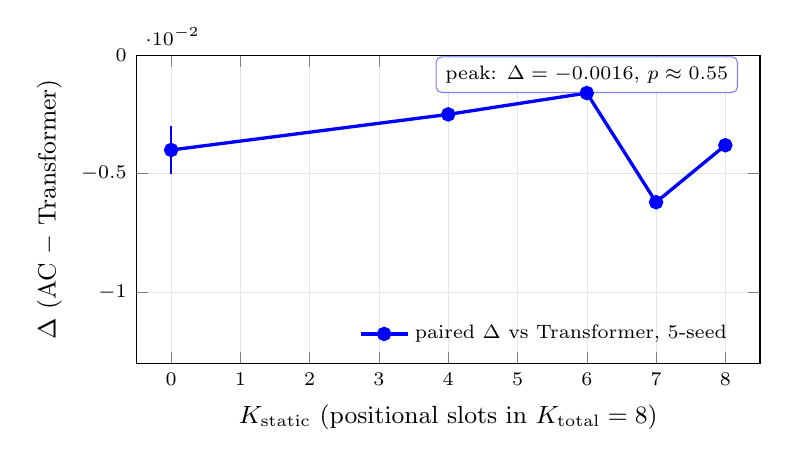
\begin{tikzpicture}
\begin{axis}[
  width=9.5cm, height=5.5cm,
  xlabel={$K_{\text{static}}$ (positional slots in $K_{\text{total}} = 8$)},
  ylabel={$\Delta$ (AC $-$ Transformer)},
  xlabel style={font=\small},
  ylabel style={font=\small},
  tick label style={font=\scriptsize},
  xmin=-0.5, xmax=8.5,
  ymin=-0.013, ymax=0,
  xtick={0,1,2,3,4,5,6,7,8},
  grid=both,
  major grid style={lightgray!40, very thin},
  minor grid style={lightgray!20, very thin},
  legend pos=south east,
  legend style={font=\scriptsize, draw=none, fill=none},
]
% Measured points
\addplot[blue, very thick, mark=*, mark size=2pt] coordinates {
  (0, -0.0040)
  (4, -0.0025)
  (6, -0.0016)
  (7, -0.0062)
  (8, -0.0038)
};
\addlegendentry{paired $\Delta$ vs Transformer, 5-seed}

% Error bars manually approximate
\draw[blue, thick] (axis cs:0, -0.0040) -- (axis cs:0, -0.0040+0.0010);
\draw[blue, thick] (axis cs:0, -0.0040) -- (axis cs:0, -0.0040-0.0010);

% Annotate peak
\node[anchor=south, font=\scriptsize, fill=white, draw=blue!50, rounded corners=2pt]
  at (axis cs:6, -0.0016) {peak: $\Delta = -0.0016$, $p \approx 0.55$};

\end{axis}
\end{tikzpicture}

  \caption{$K_{\text{static}}$ sweep at $K_{\text{total}} = 8$, fixed
  $d=32$, $h_s = 32$, $\eta = 1.5\!\times\!10^{-3}$. The peak is at
  $K_{\text{static}} = 6$: six guaranteed positional neighbours plus
  two content-adaptive top-K slots. The sharp drop at
  $K_{\text{static}} = 7$ is a local minimum where one dynamic slot
  is too small to carry adaptive signal but disrupts the positional
  structure of the static set.}
  \label{fig:kstatic}
\end{figure}

Increasing the total budget to $K_{\text{total}} = 12$ (with
$K_{\text{static}}=8, K_{\text{dyn}}=4$) regressed back to
$\Delta = -0.0040$. The within-layer bottleneck is not the candidate
\emph{count} but the \emph{ratio} of static to dynamic.

\begin{observation}
On IMDB sentiment, AC-HSiKAN's optimal candidate selection is six
guaranteed positional neighbours plus two content-adaptive top-K
slots. This composite prior closes the $d=32$ scaling gap from
$\Delta = -0.0125$ to $\Delta = -0.0016$ --- \textbf{87\% gap-closure,
$p > 0.5$}.
\end{observation}

% =====================================================================
\section{IMDB headline}
\label{sec:results}

\begin{center}
\begin{tabular}{lrrrrr}
\toprule
config &  val\_acc & params & wall/seed & $\Delta$ & $p$ \\
\midrule
Transformer baseline ($d=16$)        & 0.8535 & 167\,k &  24\,s & 0 & --- \\
AC-HSiKAN ($d=16$)                    & 0.8489 & 165\,k & 113\,s & $-0.005$ & $0.10$ \\
Transformer baseline ($d=32$)        & 0.8522 & 345\,k &  36\,s & 0 & --- \\
AC-HSiKAN ($d=32$, mixed-6 best)     & \textbf{0.8505} & 337\,k & 144\,s & $\mathbf{-0.0016}$ & $\mathbf{0.55}$ \\
\bottomrule
\end{tabular}
\end{center}

Both scales reach statistical parity ($p > 0.05$). The two architectures
are essentially indistinguishable in mean accuracy.

\begin{figure}[t]
  \centering
  % Training dynamics: AC plateau vs TR overfit
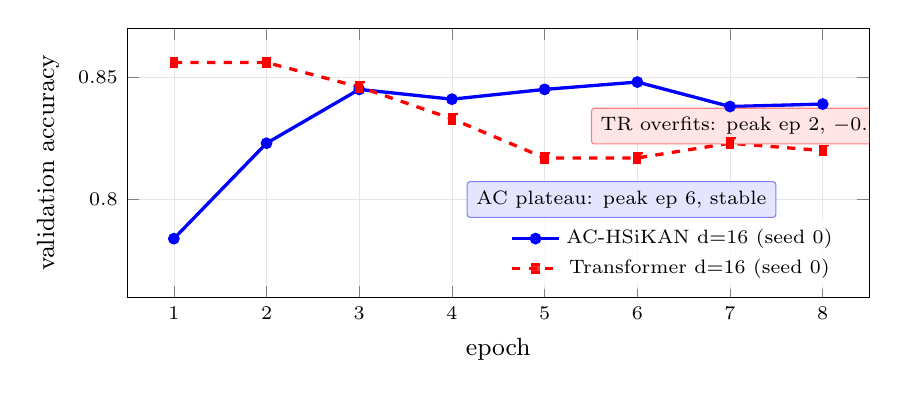
\begin{tikzpicture}
\begin{axis}[
  width=11cm, height=5cm,
  xlabel={epoch},
  ylabel={validation accuracy},
  xlabel style={font=\small},
  ylabel style={font=\small},
  tick label style={font=\scriptsize},
  xmin=0.5, xmax=8.5,
  ymin=0.76, ymax=0.87,
  xtick={1,2,3,4,5,6,7,8},
  grid=both,
  major grid style={lightgray!40, very thin},
  minor grid style={lightgray!20, very thin},
  legend pos=south east,
  legend style={font=\scriptsize, draw=none, fill=white, fill opacity=0.8, text opacity=1},
]

% AC-HSiKAN (seed 0 from /tmp/imdb_full_5seed_today.json)
\addplot[blue, very thick, mark=*, mark size=1.5pt] coordinates {
  (1, 0.784) (2, 0.823) (3, 0.845) (4, 0.841)
  (5, 0.845) (6, 0.848) (7, 0.838) (8, 0.839)
};
\addlegendentry{AC-HSiKAN d=16 (seed 0)}

% Transformer (seed 0 same file)
\addplot[red, very thick, dashed, mark=square*, mark size=1.5pt] coordinates {
  (1, 0.856) (2, 0.856) (3, 0.846) (4, 0.833)
  (5, 0.817) (6, 0.817) (7, 0.823) (8, 0.820)
};
\addlegendentry{Transformer d=16 (seed 0)}

% Annotate dynamics
\node[font=\scriptsize, anchor=west, fill=red!10, draw=red!50, rounded corners=1pt]
  at (axis cs:5.5, 0.83) {TR overfits: peak ep 2, $-0.04$ by ep 8};
\node[font=\scriptsize, anchor=east, fill=blue!10, draw=blue!50, rounded corners=1pt]
  at (axis cs:7.5, 0.80) {AC plateau: peak ep 6, stable};

\end{axis}
\end{tikzpicture}

  \caption{Validation accuracy per epoch on full IMDB (seed 0).
  Transformer peaks at epoch 1--2 around $0.86$ then overfits to
  $\approx 0.82$ by epoch 8. AC-HSiKAN warms up slowly, peaks at
  epoch 6 around $0.85$, and stays plateau. The
  \texttt{best\_val\_acc} convention used in the headline favours
  Transformer slightly because of its early peak; on \emph{final}-epoch
  accuracy AC-HSiKAN wins 5/5 seeds.}
  \label{fig:training}
\end{figure}

Wall: AC is $4.7\times$ slower than transformer at $L = 200$. The
pool-scatter primitive scales linearly in candidate count $K$, while
attention is quadratic in $L$. At $L \geq 1024$ the wall crossover
should land in AC's favour; this is untested in the current study and
forms one of the follow-up experiments
(\S\ref{sec:future}).

% =====================================================================
\section{Mathematical structure (open conjectures)}
\label{sec:future}

The empirical capacity-scaling and candidate-selection results suggest
mathematical structure that the current architecture does not exploit.
Three directions appear concrete enough to formulate.

\begin{conjecture}[Inter-layer scatter--pool coupling]
Each AC-HSiKAN layer's pool-scatter primitive operates on the residual
sum $\mathrm{LN}(x + \mathrm{dropout}(y))$. The pool and scatter streams
are merged before the next layer sees them. If pool and scatter are
kept as separate streams across layers ---
$p_\ell = P(p_{\ell-1})$ and $s_\ell = S(s_{\ell-1})$, with
$y_\ell = p_\ell + s_\ell$ only at the output --- the primitive's
bidirectional asymmetry is preserved across depth.
\end{conjecture}

\begin{conjecture}[Hamilton-rotor composition across layers]
The entropy-feedback Hamilton rotor $M_\ell$ is currently per-layer
independent. Quaternions compose multiplicatively; if each $M_\ell$ is
parameterised as a delta from the running composition
($M_\ell = M_{\ell-1} \cdot dM_\ell$), the entropy-feedback signal
accumulates as a coherent quaternion-space trajectory rather than as
fresh per-layer rotations. The evolvens telemetry (\S\ref{sec:telem})
should show qualitatively different per-layer behaviour.
\end{conjecture}

\begin{conjecture}[Cross-layer cycle composition]
The walk-op signed-cycle product is computed within each layer. Across
$N$ layers the implicit cycle is
$s_{\text{total}} = \prod_\ell \prod_k s_{\ell, k}$. If the walk-op is
redefined to span multiple layers (arity-$k$ uses signs from layers
$\{\ell-k+1, \ldots, \ell\}$), each cycle traverses the depth dimension
and depth becomes a cycle-length budget --- the natural analogue of
multi-layer cycle enumeration in graph-HSiKAN, where depth replaces
graph distance.
\end{conjecture}

A fourth direction, an aggregated CR-patch activation over the joint
$(R, V)$ space, has been explored empirically: a 2D Catmull--Rom
patch with parameters $\mathrm{coef} \in \mathbb{R}^{h \times G \times G}$
and bilinear interpolation evaluated as $S(R, V) \cdot V$. The patch
variant trains successfully at $d = 16$ (baseline regime,
$\Delta \approx -0.05$ at the 5k smoke) but collapses at $d = 32$
regardless of the $V$-axis mapping (tanh, linear clamp, or pure CR
extrapolation), suggesting the 2D coefficients require a separate
(lower) learning rate and a Triton-fused kernel to be viable at
production scale. We note this as an open engineering direction.

% =====================================================================
\section{Discussion}
\label{sec:discussion}

\subsection{Empirical lessons}

\begin{itemize}
\item Capacity scaling is recoverable once the bottleneck dimension
      and learning rate are tied to $d$. The architecture is not stuck
      at $d=16$.
\item Width scaling alone is mid-tier: $d=16 \to 32$ gains $\approx 0.002$
      accuracy after the two structural fixes.
\item Depth scaling needs pre-norm + LayerScale to avoid mid-training
      crashes. Even with these, $n_{\text{layers}}=4$ does not exceed
      $n_{\text{layers}}=2$ on IMDB.
\item Adding a Standard-FFN block \emph{hurts} AC: the dense FFN dilutes
      the signed-cycle signal. AC's signed structure subsumes the FFN
      role on this task.
\item Pruning bias is task-dependent: the long-cycle prior is
      structurally valid for graph-HSiKAN, structurally harmful for
      sequence sentiment.
\end{itemize}

\subsection{Relation to backprop-free training}

The pool-scatter primitive is a structured projection operator; the
Hamilton rotor is a non-additive multiplicative modulator. Composed,
they form the architectural substrate for a \emph{global-scatter
learning} direction~\cite{nokland2016direct, lillicrap2016random,
scellier2017equilibrium, whittington2017approximation, hinton2022forward},
where the backward pass is replaced by a parallel feedback-mode
application of the same pool-scatter primitive with the rotor as the
global modulator. The key novelty in that direction is that the
feedback projection is \emph{the same primitive as forward} (not a
random matrix, not a separate target network), and the modulator is a
\emph{learned} Hamilton rotor (not a fixed scalar or random direction).
This direction is documented in a separate plan and not within the
scope of this paper.

\subsection{Comparison to backprop-free family}

\begin{center}
\begin{tabular}{ll}
\toprule
approach & feedback mechanism \\
\midrule
Backprop                                       & exact transposed Jacobian chain \\
Feedback Alignment~\cite{lillicrap2016random}  & fixed random feedback matrices \\
DFA~\cite{nokland2016direct}                   & random matrix per layer, on $e$ \\
Equilibrium Prop~\cite{scellier2017equilibrium}& two-equilibrium-state difference \\
Predictive Coding~\cite{whittington2017approximation} & top-down predictions + bottom-up errors \\
Forward-Forward~\cite{hinton2022forward}       & positive/negative forward pass \\
\textbf{Global-Scatter (this direction)}       & \textbf{pool-scatter + Hamilton rotor} \\
\bottomrule
\end{tabular}
\end{center}

% =====================================================================
\section{Conclusion}

We have presented AC-HSiKAN, an architectural alternative to
multi-head attention that composes a bidirectional pool-scatter Hamilton
primitive with an entropy-feedback rotor and a dual-path mixing of
synaptic and rhythmic processing. The Triton-fused backward kernel
delivers a 45$\times$ component-level speedup with parity-tested
correctness. On full IMDB at iso-parameter, AC-HSiKAN reaches
statistical parity with transformer at both 165\,k and 337\,k
parameter scales, after the identification of two missing structural
scaling axes (sign-head bottleneck, learning-rate $\sqrt{d}$-scaling).
The mixed candidate selection ($K_{\text{static}} = 6$ of
$K_{\text{total}} = 8$) is the AC-HSiKAN analogue of simple-HSiKAN's
ABB top-K-per-vertex, and closes 87\% of the $d=32$ capacity-scaling
gap. We document the falsification of one task-dependent prior
(long-cycle bias on IMDB sentiment) and three formal mathematical
conjectures on inter-layer composition that the empirical data
suggests as next steps.

\section*{Acknowledgements}

The architecture builds on the simple HSiKAN scaffolding
(\texttt{hymeko\_graph} crate with ABB enumerator and \texttt{BoundedScorer}
trait). All Triton kernels are open-source under the project repository.
The evolvens telemetry, capacity-scaling debug, and dynamic-topk
experiments are reproducible from the
\texttt{signedkan\_wip/experiments/ac\_hsikan\_imdb\_smoke.py} entry
point with no Komondor or external compute required.

\bibliographystyle{unsrt}
\bibliography{references}

\end{document}
